\documentclass[12pt]{report}%{memoir}

\usepackage[utf8]{inputenc}
\usepackage[T1]{fontenc}
\usepackage[english]{babel}

\usepackage[a4paper]{geometry}  % Pour indiquer le format de page

% Pour la bibliographie
\usepackage[backend=biber,style=reading,sorting=nyvt]{biblatex}
\bibliography{Bibliographie}

\usepackage[style=french]{csquotes}

% Pour les liens
\usepackage{hyperref}
\hypersetup{
    colorlinks,
    citecolor=black,
    filecolor=black,
    linkcolor=black,
    urlcolor=blue
}

% Pour que les figures apparaissent sur la bonne page
\usepackage{float}

\usepackage{verbatim}

% Pour les annexes
\usepackage[toc,page]{appendix}

% Pour les images
\usepackage{graphicx}

%Multiple figures
\usepackage{subcaption}

\title{\textbf{LO53 Wi-Fi Positioning System\\ Lab report}}
\author{Thomas Gagneret\\ Stéphane Parunakian\\ Tao Sauvage}
\date{}

\begin{document}

\maketitle

\input{introduction.tex}

\setcounter{tocdepth}{1}
\tableofcontents

\chapter{Access Points}

A main component of the project concerns the access points configuration. In
this chapter, their features will be described.

\section{Chained list of the UEs}

The access point will use a chained list in order to save the different
measures retrieved from the UEs' Wi-Fi signals.

With this datastructure the AP is able to manage an infinite number of UEs. For
each of save, it will save its MAC address and its corresponding RSSI value.

It also provides two functions, \emph{build\_element} and \emph{build\_buffer},
that will convert the chained list into JSON data that will be later send to
the Positioning Server.

\section{Passive Sniffer}

Now that the AP has a list, it then needs to fill it with the different values.

In order to find the MAC addresses and the RSSI values of each device, it needs
to sniff the network for any Wi-Fi signals sent by it.

The AP achieve this sniffing by using the \emph{PCAP} library.

It first set up a hook on its interface in order to intercept any Wi-Fi packets
on the network like below.

\begin{figure}[h]
  \centering
  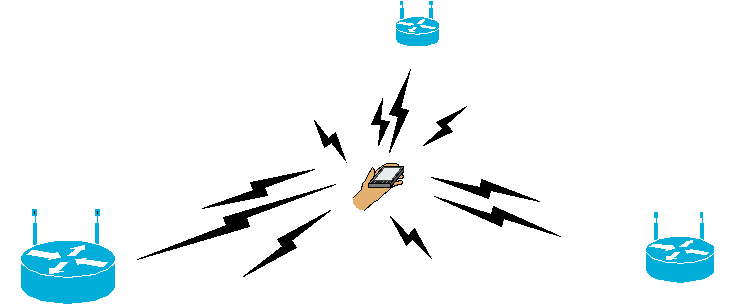
\includegraphics[scale=.5]{./ap/mobile_with_aps.png}
  \caption{Each AP sniffs the Wi-Fi packets of the network}
\end{figure}

Then for each packet, it extracts the MAC address and the RSSI value fields.

\begin{figure}[h]
  \centering
  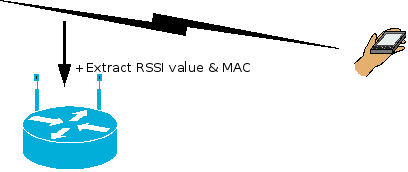
\includegraphics[scale=.7]{./ap/focus_mobile_with_aps.png}
  \caption{For each packet, the AP extracts two fields}
\end{figure}

It sets up a
hook on its interface and extract form the sniffed packets two fields: the MAC
address and the RSSI value.

It then create a new list element with these two values.

\section{HTTP Daemon}

At this point, the AP is able the measure every RSSI values for any devices on
the network. It then has to be able to send them to the Positioning Server when
asked.

Therefore the AP creates a HTTP daemon using the \emph{MicroHTTP} library.

When being fired up, it will initialize that daemon using the
\emph{start\_microhttpd} function. As a callback function, the AP will pass the
\emph{connection\_callback} one that will react to a \emph{?mac=} HTTP request.

It will then uses the list's functions in order to create the JSON response and
sends it to the PS.


\chapter{Positioning server}

In this chapter, we will speak about the positioning server part of our project. 

    \section{Tools and versions}

Before seeing the server itself, lets see the different tools used for its
creation.

        \subsection{Java}

This server is coded in Java 7, the programming language of Oracle. So the
different servlets must use TomCat 7.

%        \subsection{Git}

        \subsection{Simulation scripts}

In order to test the server, without having to setup all the elements of the
project (Access points, mobile device), three Python scripts have been written:

\begin{description}
    \item [AccessPoint] Simulate the response of an access point.
    \item [MobileDevice (Calibration)] Simulate the calibration request of a
        mobile device.
    \item [MobileDevice (Localisation)] Simulate the localisation request of a
        mobile device.
\end{description}

    \section{Programm}

Now we will look at the server.

        \subsection{DAO}

A major element of the server code is the Data Access Object (DAO). It is the
link between the database and the code. It allows the programm to manipulate
data as it was objects, without having to care about the database. The DAO
creates objects from information in the database, and updates information in the
database from objects.

The major advantage of this concept is the possibility to change the way to
store data easily. Only the DAO interface needs to be modified in case we want,
for example, to use a NoSQL database.

        \subsection{Calibration}

The Calibration servlet is called by mobile devices to put calibration information
in the server database.

How the servlet works:
\begin{enumerate}
    \item A mobile device send a calibration request, with a map id and
        coordinates.
    \item The servlet get a list of all routers present in database.
    \item If there is enough routers, it goes on, else it stops.
    \item It sends RSSI requests to router and wait no more than 500 ms for the
        response.
    \item If there is enough useful responses, it stores them in the database
        (RSSI table), else it stops.
    \item It sends a response to the mobile device.
\end{enumerate}

        \subsection{Localisation}

The Localisation servlet is called by mobile devices who want their
localisation.

How the servlet works:
\begin{enumerate}
    \item A mobile device send a localisation request, with no parameters.
    \item The servlet get a list of all routers present in the database.
    \item If there is enough routers, it goes on, else it stops.
    \item It sends RSSI requests to router and wait no more than 500 ms for the
        response.
    \item If there is enough useful responses, it stores them in the database
        (TempRSSI table), else it stops.
    \item It gets every location calibrated from the database and calculate the
        distance with the data in the TempRSSI table, for each location.
    \item It returns the closest location to the mobile device (map id,
        coordinates).
\end{enumerate}

%        \subsection{Other}

    \section{Database}

The database of the server is shared between the servlets. Its structure is
almost the same as in the subject. There is only one addition: an ``ip'' column
in the AccessPoints table (it is more reliable than using the id for the last
part of the ip).

\begin{figure}[h]
  \centering
  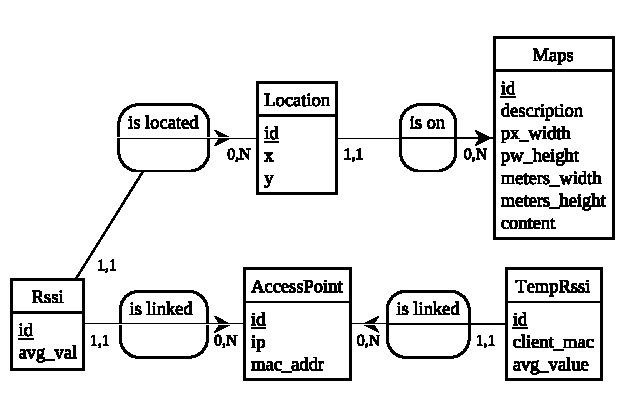
\includegraphics[scale=1]{./positioning_server/db.pdf}
  \caption{Database}
\end{figure}

        \subsection{Creation script}

In order to create the database, a postgresql script has been created. It
creates a user ``lo53'' with a password ``lo53'' and a database ``lo53\_rssi''.

        \subsection{Filling}

The filing of the database has to be handmade, except for the Maps table. As
this table contains binary data, it is quite difficult to do it manually. So we
wrote a filling script to do this. This script put maps pictures in the
database, and get informations about maps from text files like this one :

\verbatiminput{./positioning_server/pic.txt}

The size in pixel of the picture is automatically determined, thank to the PIL
library. The addition in the database uses the psycopg2 connector.


\chapter{Android}
In this chapter we will talk about the two applications used by the different users to communicate with the server.

\section{Settings}
First, for this two applications we designed a preference activity which allows the user to change different values to access the server. Indeed the address, the port and the servlet to use can be changed.

\begin{figure}[h!]
  	\centering
    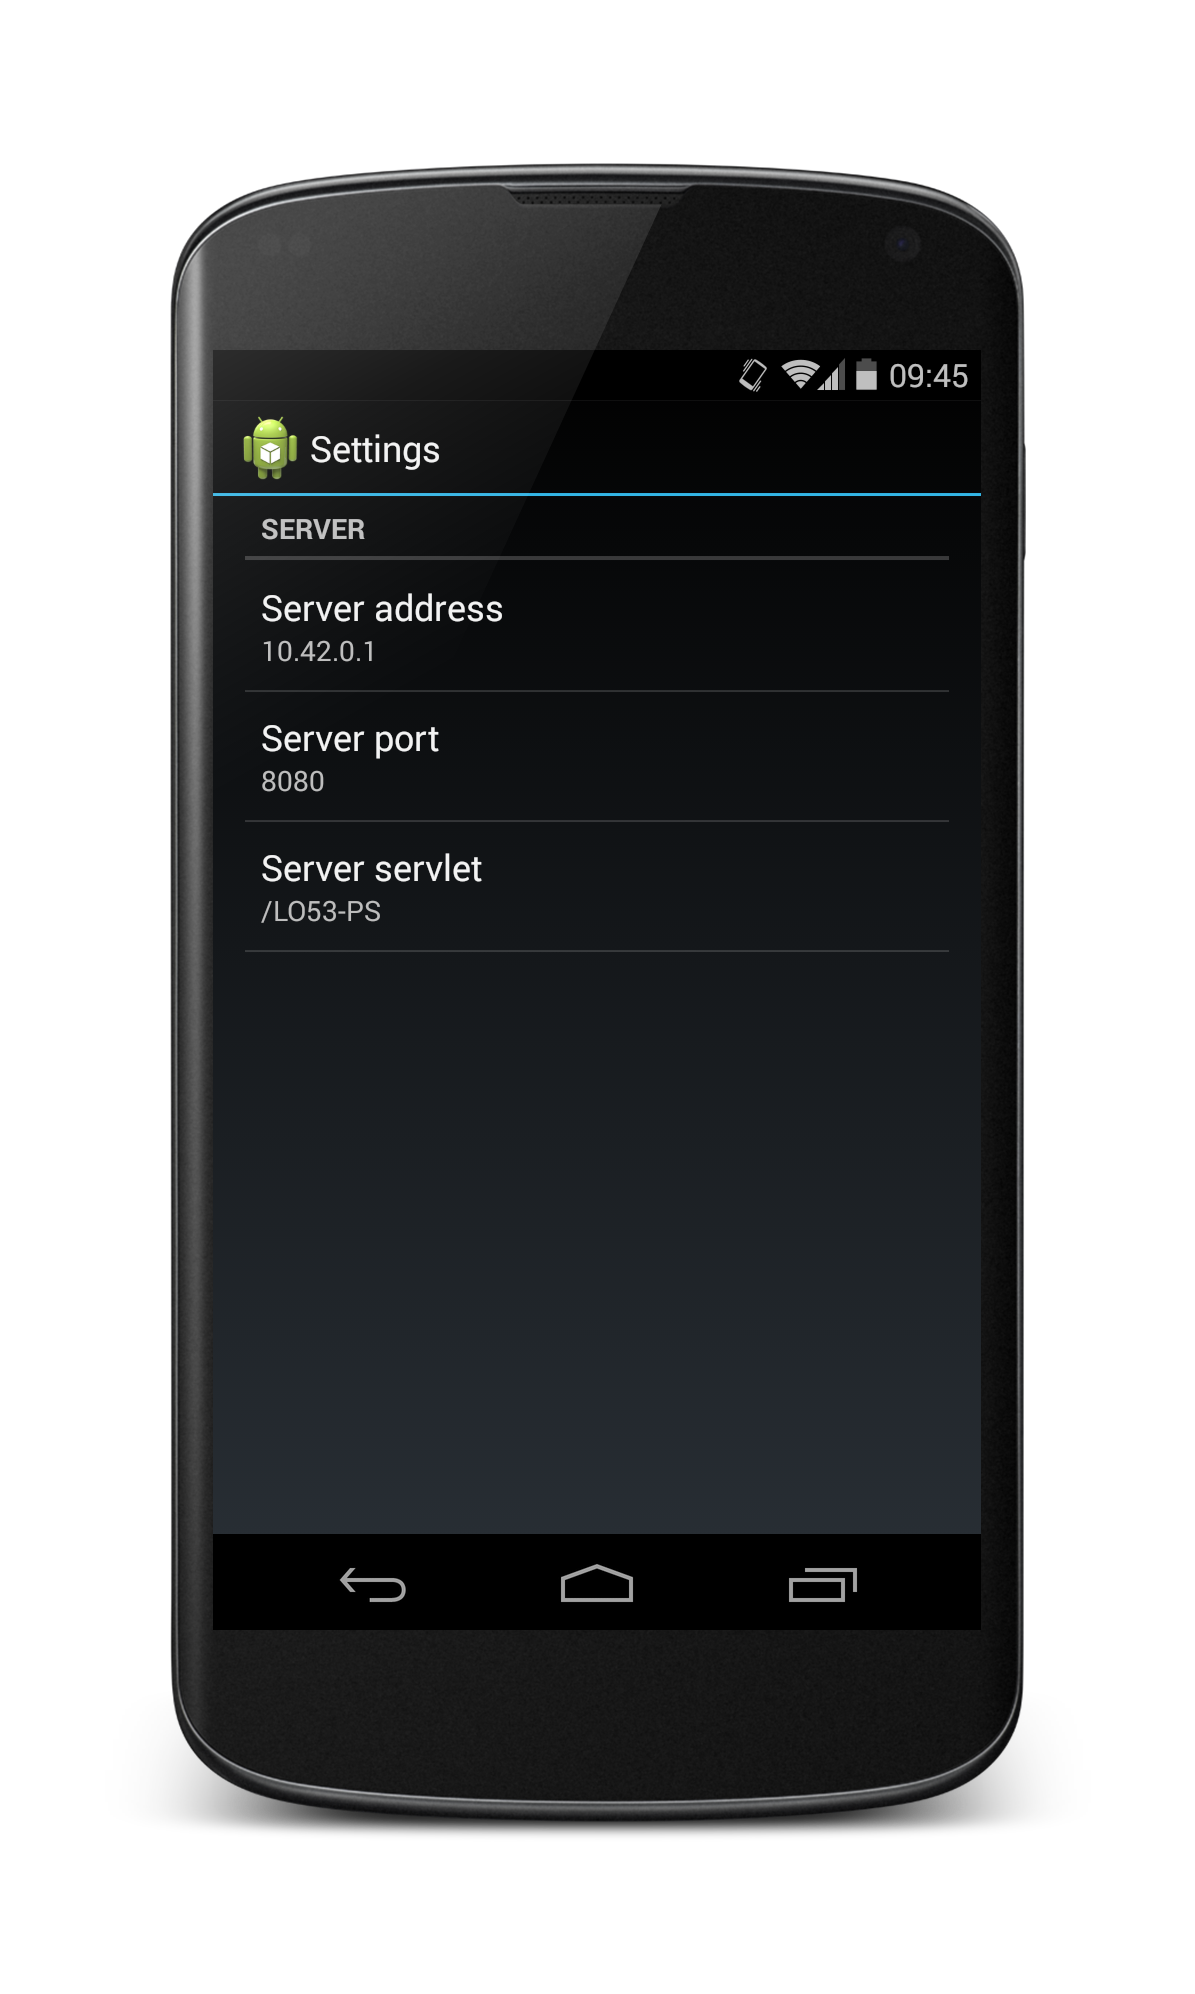
\includegraphics[scale=0.1]{./android/Settings.png}
  \caption{Settings activity}
\end{figure}


\section{Setup Tool}
Now, we will talk about the setup tool application which allows a network administrator for example to set some calibration points in the building. On the next figure you can see the different phase to use this application.


\begin{figure}[h]
        \centering
        \begin{subfigure}[b]{0.3\textwidth}
    			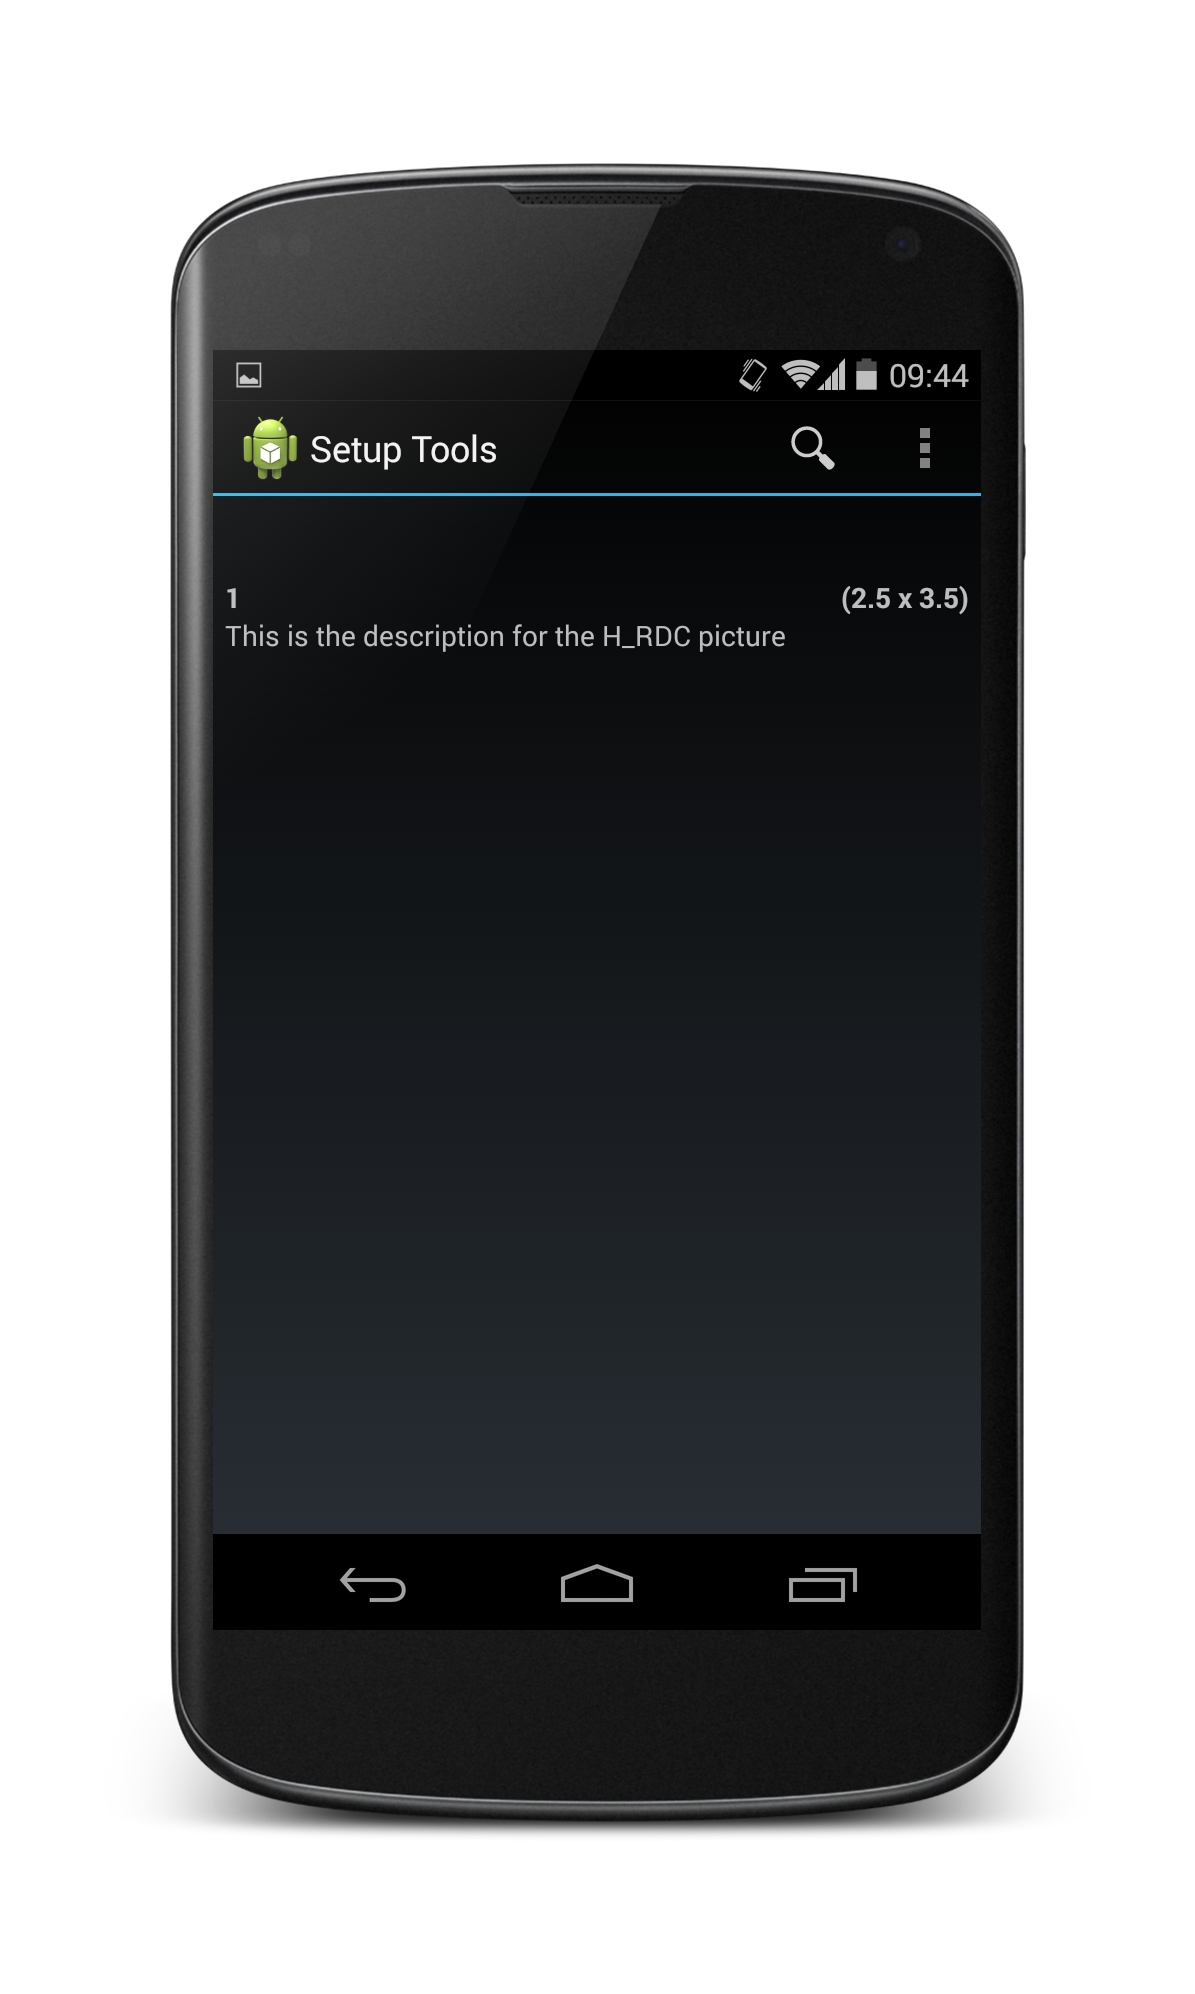
\includegraphics[scale=0.1]{./android/Setup_list.png}
                \caption{Choose your map}
                \label{fig:map_list}
        \end{subfigure}
        \begin{subfigure}[b]{0.3\textwidth}
                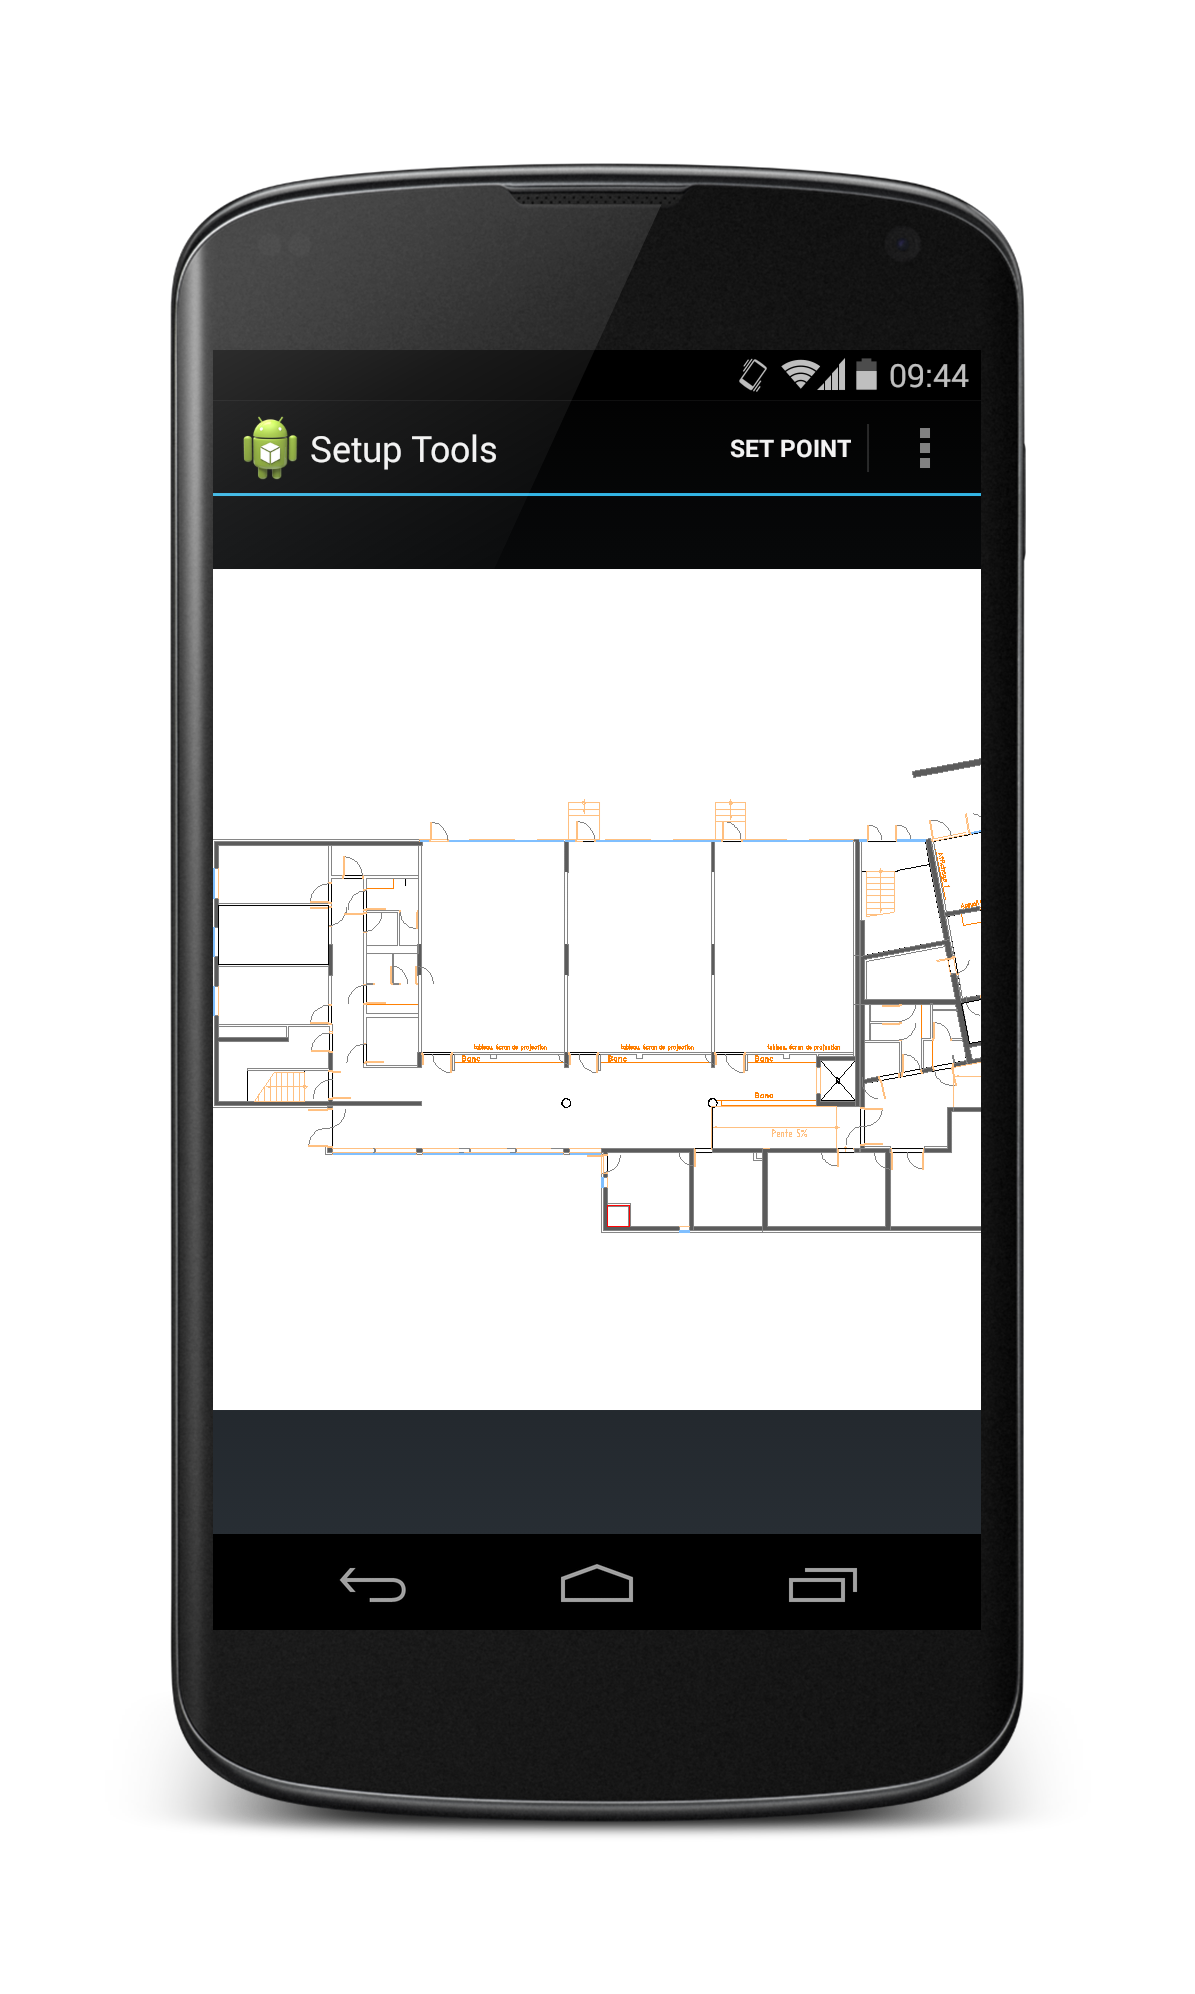
\includegraphics[scale=0.1]{./android/Setup_set.png}
                \caption{Display the map}
                \label{fig:map_set}
        \end{subfigure}
        \begin{subfigure}[b]{0.3\textwidth}
                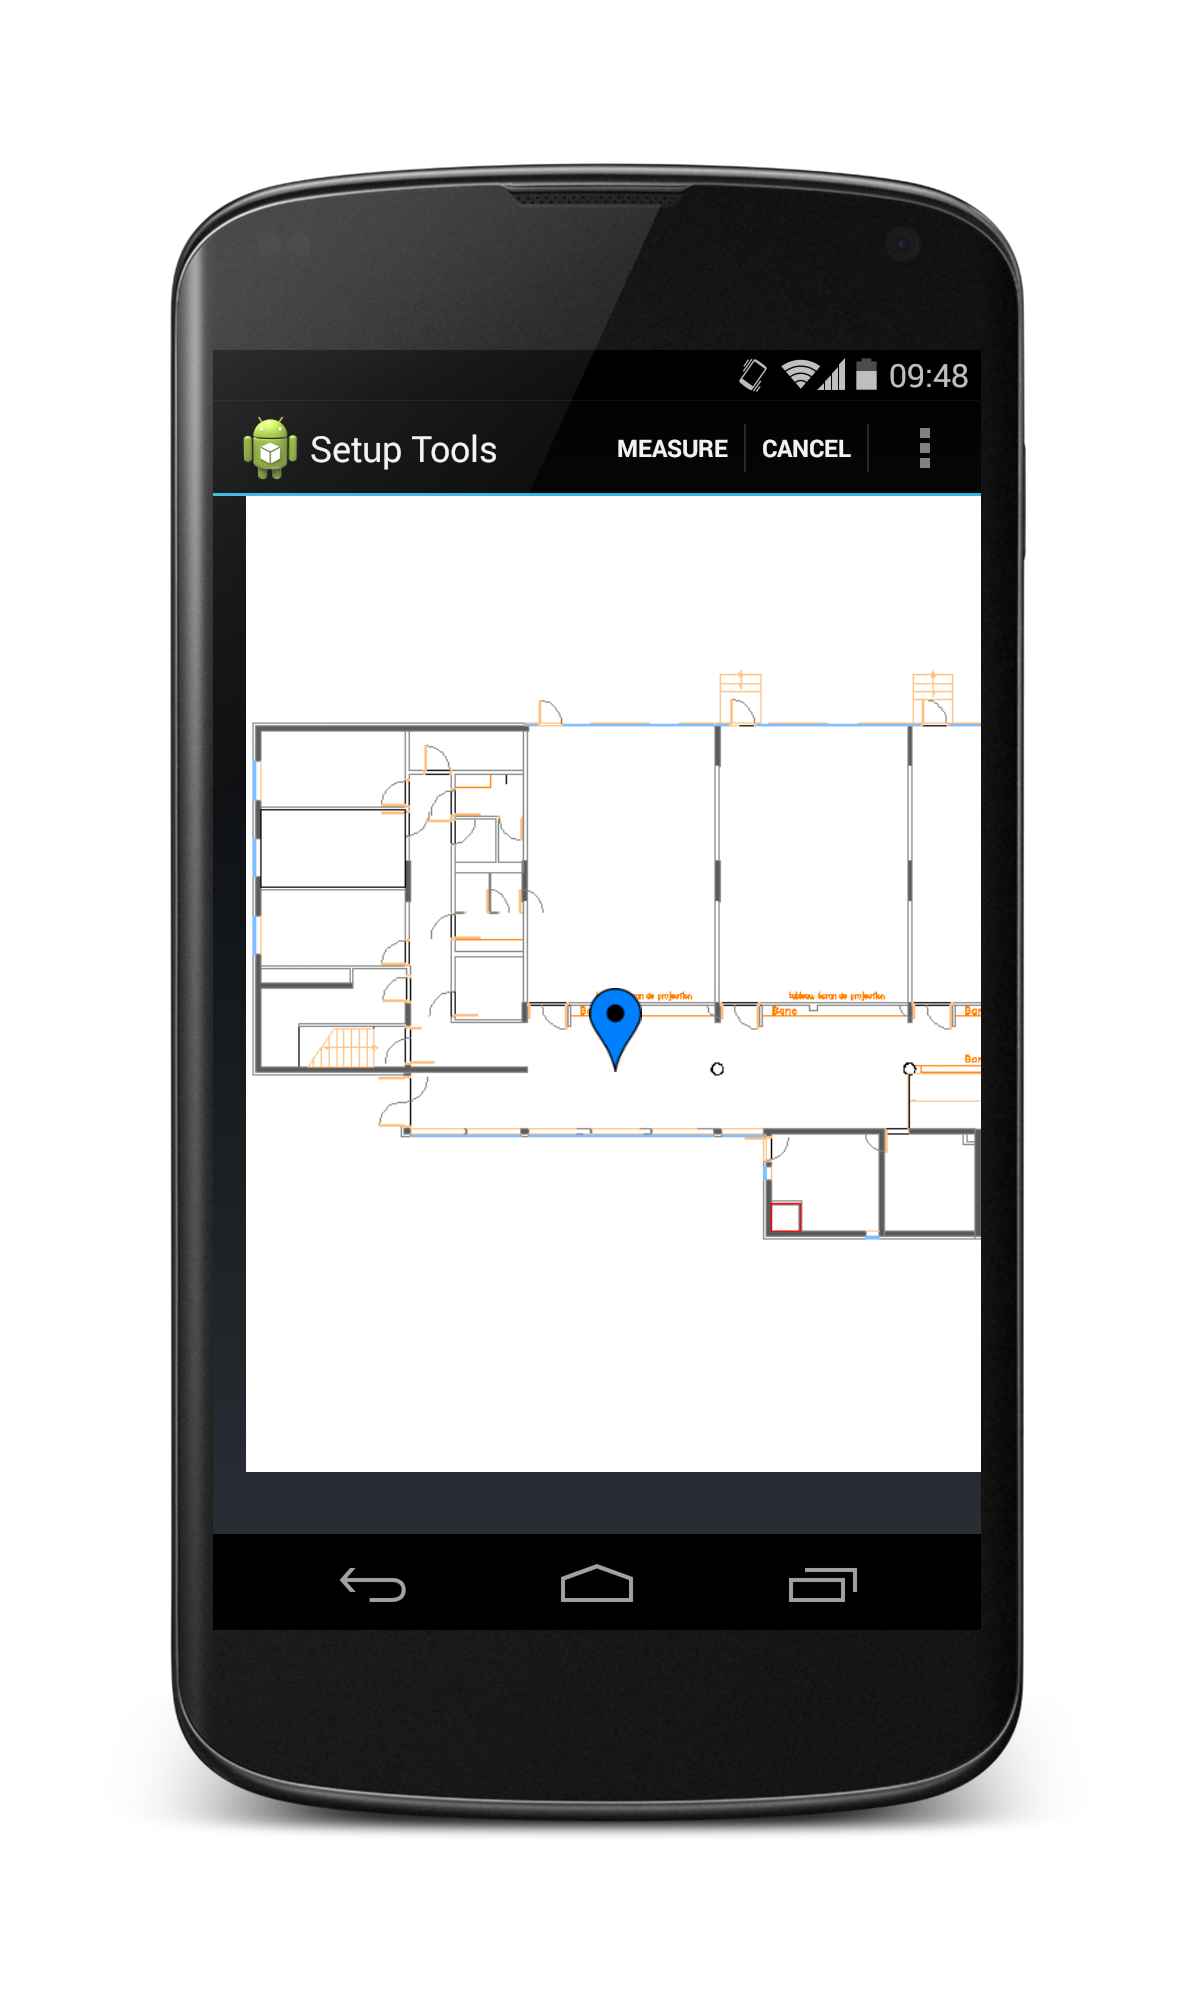
\includegraphics[scale=0.1]{./android/Setup.png}
                \caption{Set calibration point}
                \label{fig:map}
        \end{subfigure}
        \caption{Setup Tools application}\label{fig:setup}
\end{figure}

\begin{itemize}
\item First, when you launch the application there is a list of all map available on the server which is displayed. It contains the id, a description and the size of the map in meters. Then you just have to select the correct one. It is also possible, when you know the id of the map to use the search bar. Indeed you just have to put the correct id and it will display the map just like if you choose it from the list. (See Figure \ref{fig:map_list})
\item Then when the map is displayed you have to click on the "set" button to be able to add a calibration point. (See Figure \ref{fig:map_set})
\item Once you clicked on the "set" button you can set your calibration point and click on "measure" to send all the information to the server. It's also possible to cancel using the "cancel" button which remove your calibration point (on the map). (See Figure \ref{fig:setup})
\end{itemize}

\section{Positioning}
Now we will talk about the positioning application which allow a user to be located in a building according to the calibration points set with the previous application.

\begin{figure}[h!]
  	\centering
    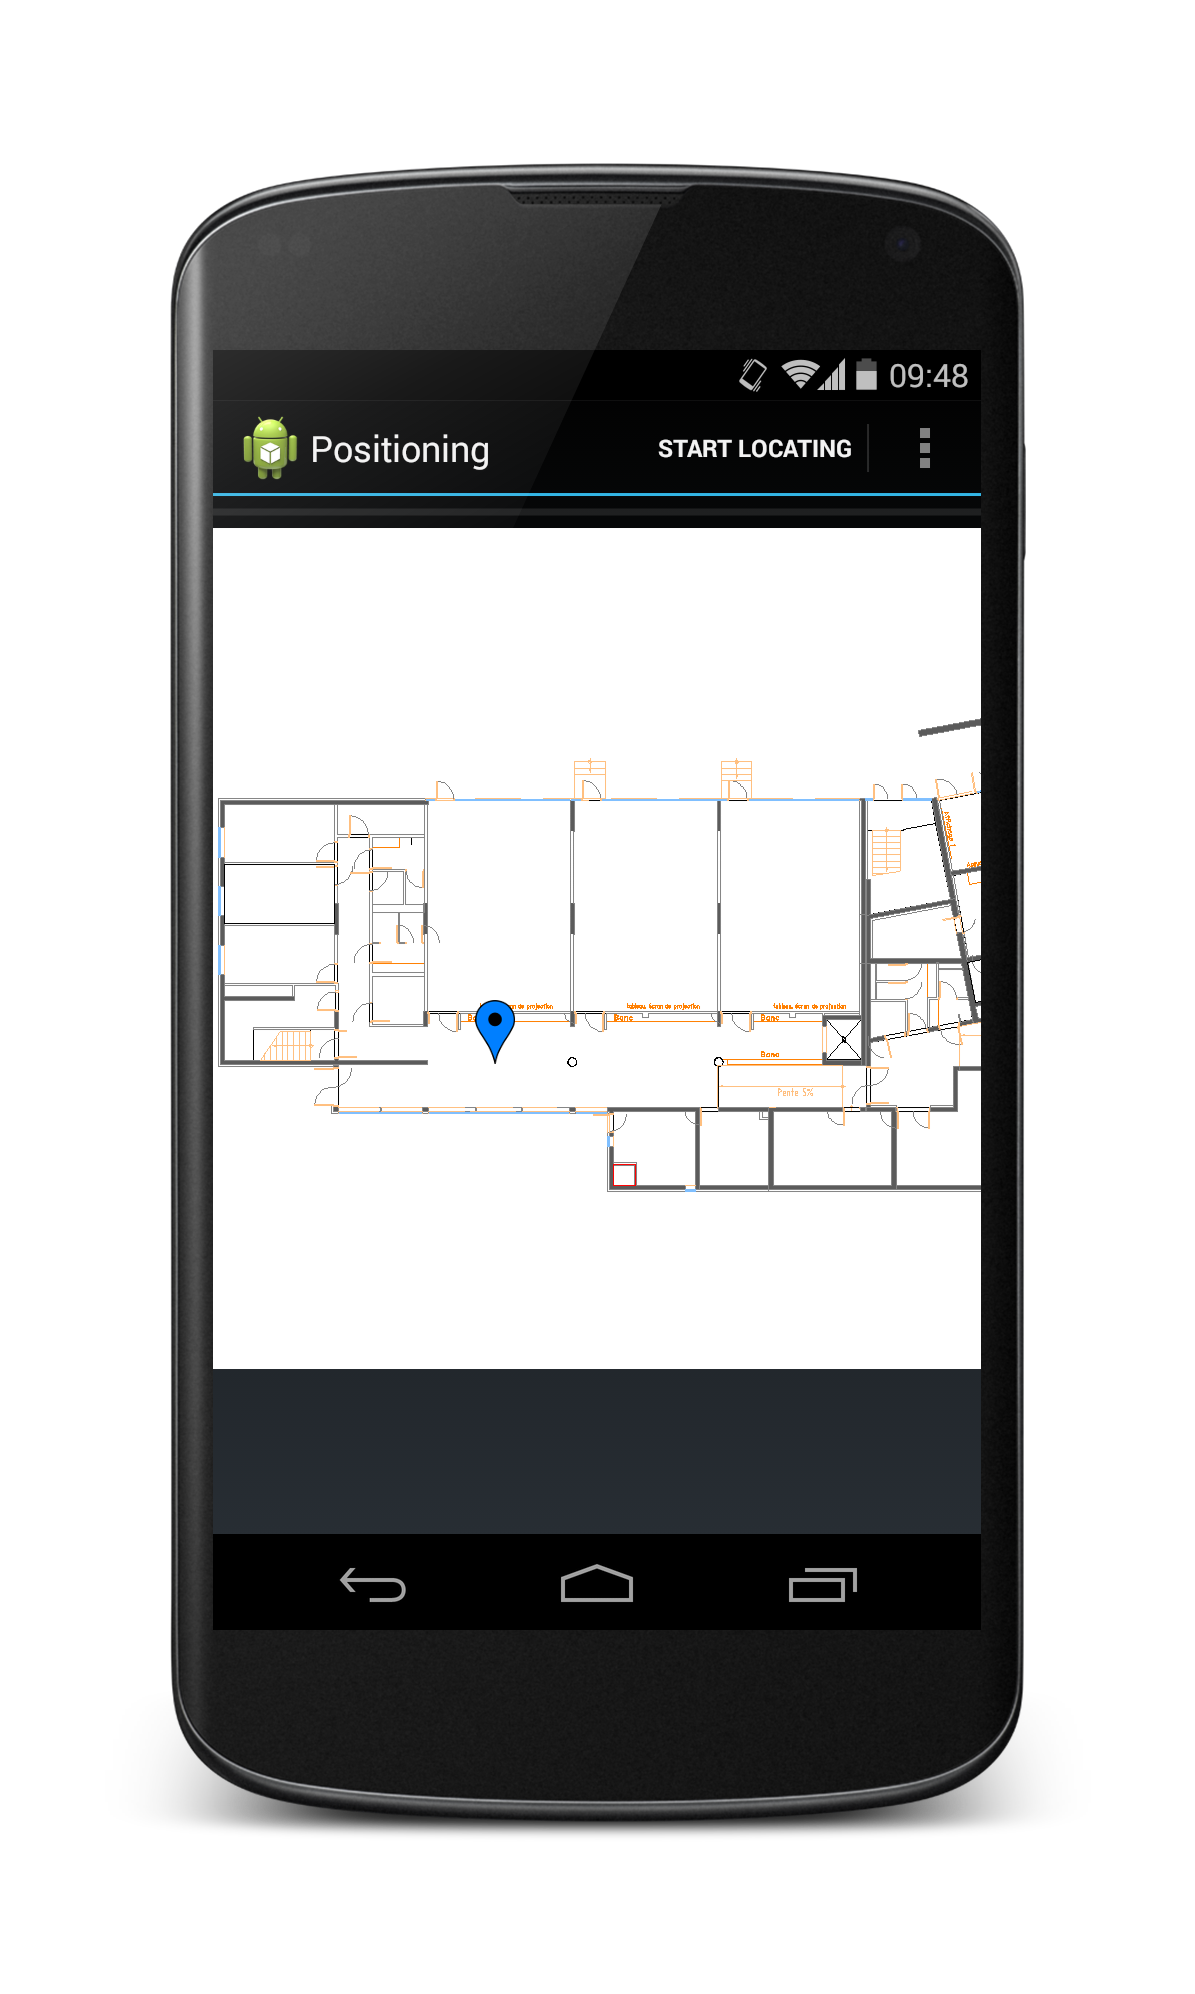
\includegraphics[scale=0.1]{./android/Positioning.png}
  \caption{Positioning application}
\end{figure}

This application is very simple. The user just have to click on "Start locating" and the application sends a positioning request to the server and display the result on the screen (map to display, position).


\section{RSSI values}

For this two applications the access points require a maximum of RSSI values. If the mobile does not communicate, the access points do not retrieve RSSI values which prevents the applications to work correctly. So in both application we ping the server but also launch a wifi scan which allow the access points to retrieve about 50 RSSI values.



\input{./conclusion.tex}

%\nocite{*}

%\printbibliography[heading=bibintoc]

\newpage
\thispagestyle{empty}
\null
\vspace{\fill}
\begin{center}
    
\includegraphics[width=1in]{./license.png} \\
    This report is licensed under a Creative Commons Attribution 4.0
    International License.
\end{center}


\end{document}
